\begin{frame}{Реализация упрощённой системы}
    \begin{itemize}
        \item Нужна для лучшего понимания, как работает Nanite
        \item Преобразование меша в граф --- долгий предподсчёт
        \item Разбиение меша с помощью библиотеки METIS
        \item Невозможно задать жёсткое ограничение на размер мешлета, поэтому количество мешлетов берётся с запасом
        \item Реализован алгоритм уменьшения детализации, т.к. библиотеки работают с целым мешем
        \item Отрисовка --- Mesh Shader в DirectX 12
        \item Обход всего графа для упрощения
    \end{itemize}
\end{frame}

\begin{frame}{Реализация: скриншоты}
    \begin{center}
        Разные настройки допустимого искажения для наглядности

        \medskip

        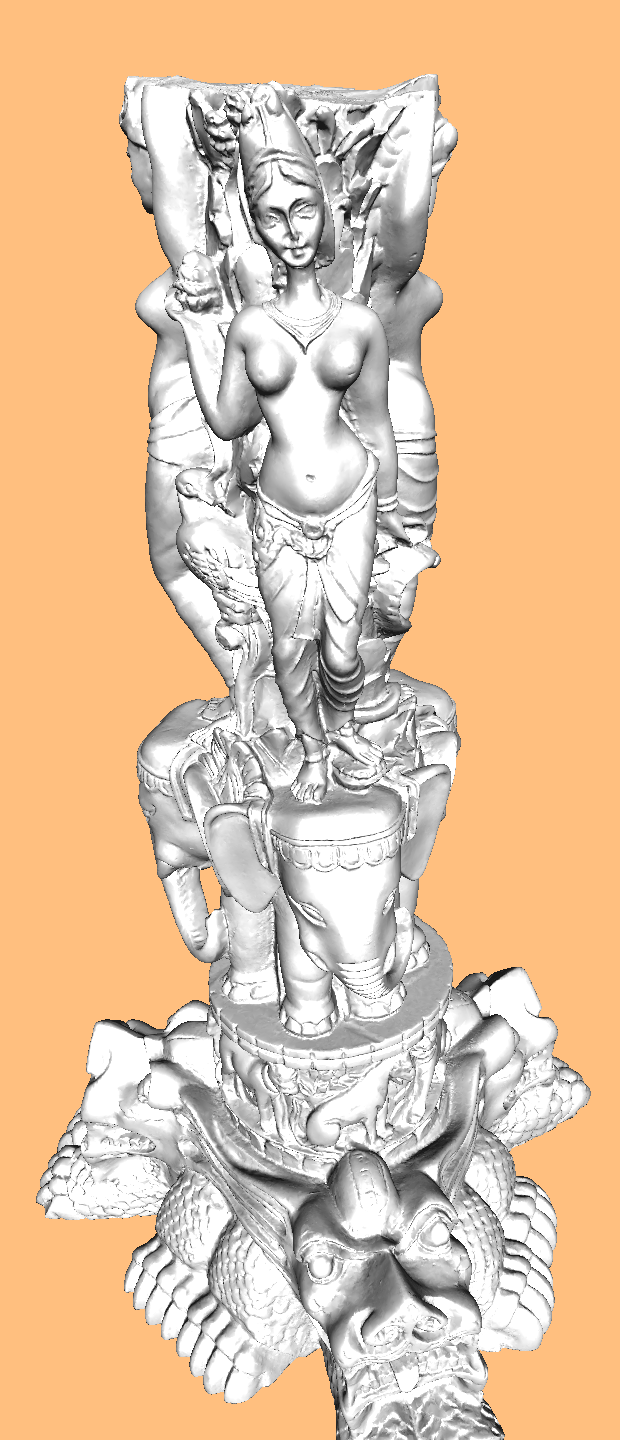
\includegraphics[width=.2\textwidth]{pics/demo-cut-0.png}
        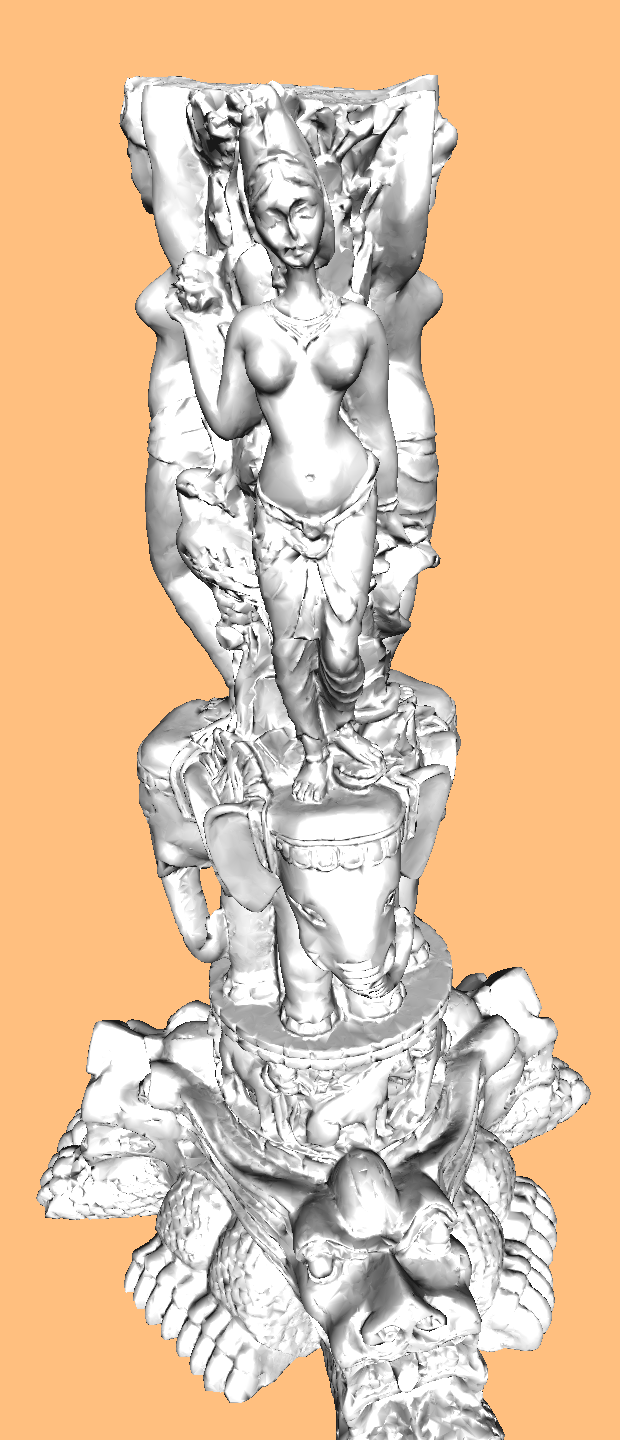
\includegraphics[width=.2\textwidth]{pics/demo-cut-1.png}
        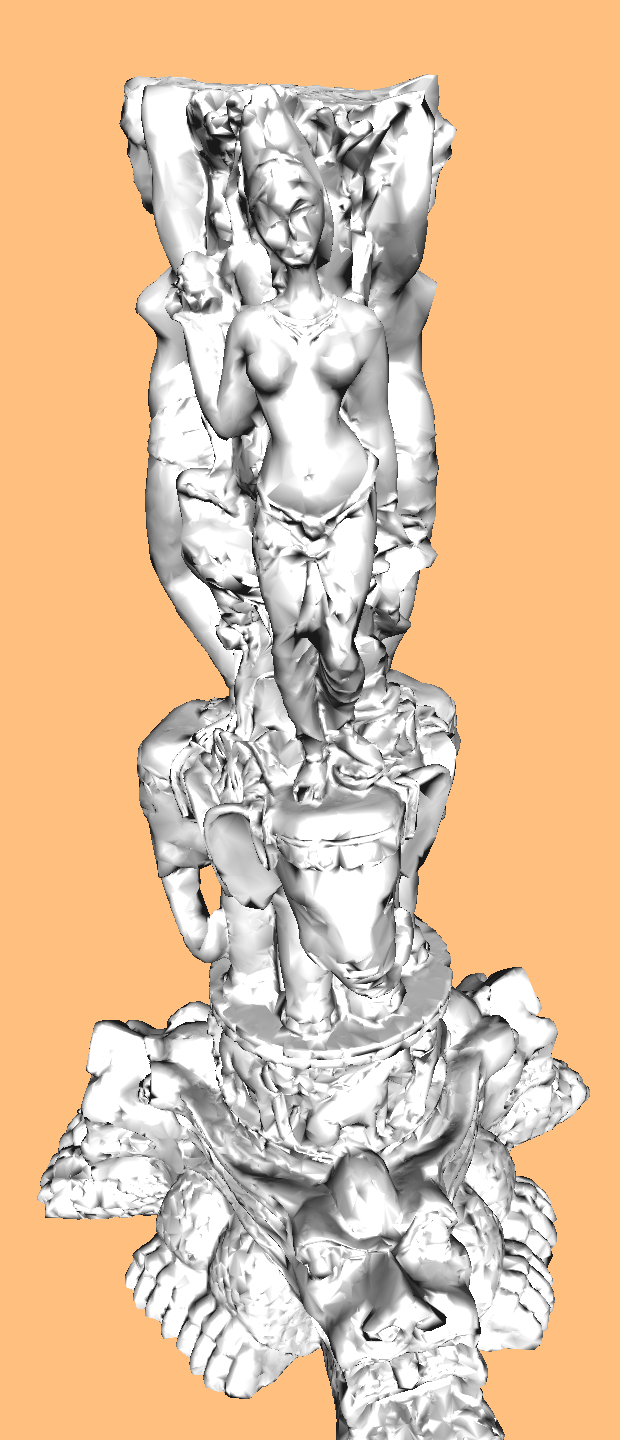
\includegraphics[width=.2\textwidth]{pics/demo-cut-2.png}
        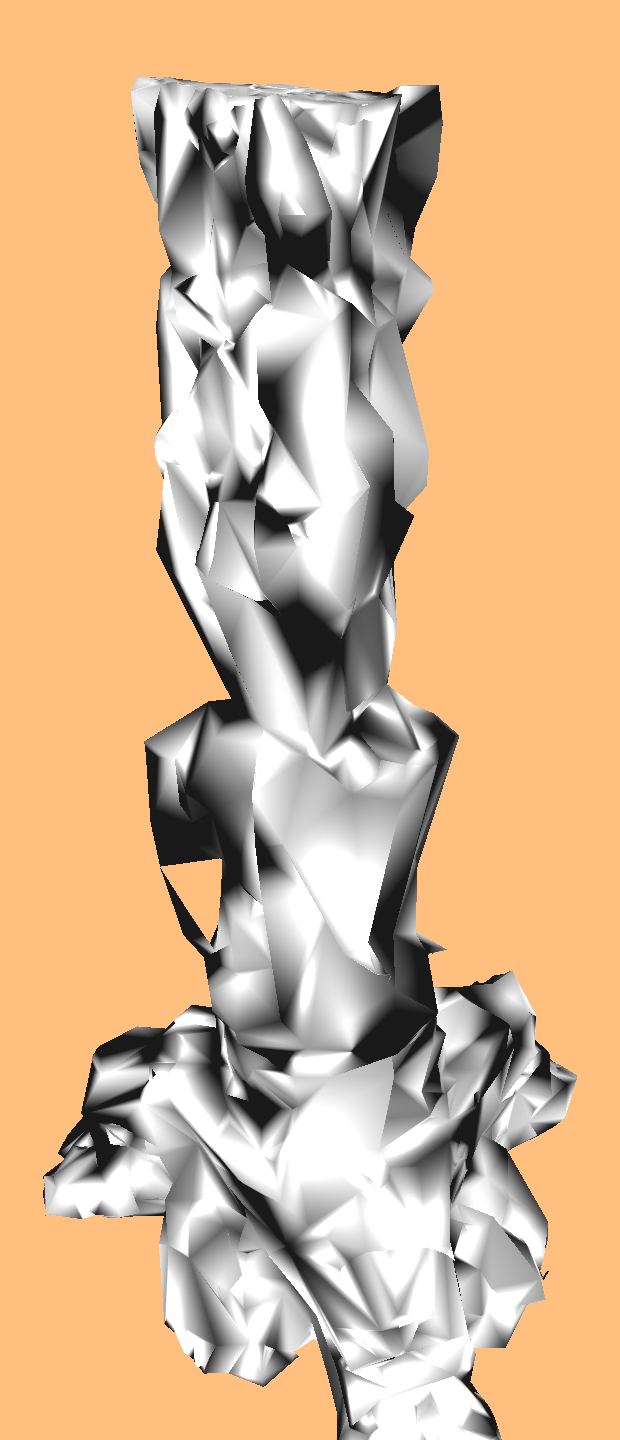
\includegraphics[width=.2\textwidth]{pics/demo-cut-3.png}

        \parbox[l]{.4\textwidth}{
            Вид вблизи
        }
        \parbox[r]{.4\textwidth}{
            \hfill
            Вид вдали
        }
    \end{center}
\end{frame}
